\documentclass[12pt,a5paper,titlepage, main = russian]{article}
\usepackage[T1,T2A]{fontenc}
\usepackage[utf8]{inputenc}
\usepackage[warn]{mathtext}
\usepackage{textcomp}
\usepackage[russian]{babel}
\usepackage{extsizes}
\usepackage[left = 1 cm, right = 1 cm, top = 1.5 cm, bottom = 1.5 cm]{geometry}
\usepackage [pagestyles, raggedright]{titlesec}
\usepackage{graphicx}
\usepackage{ragged2e}
\usepackage{amsmath}
\usepackage{pgfplots}
\pagestyle{empty}
\usepackage{tikz}
\usetikzlibrary{patterns}

\usepackage{wrapfig}

\usepackage{siunitx} % Required for alignment
\usepackage{multirow}
\usepackage{rotating}
\usepackage{float}
\usepackage{booktabs}

\usepackage{amsmath,amsfonts,amssymb,amsthm,mathtools} % AMS
\usepackage{icomma}
\usepackage[russian]{babel}
\usepackage[T2A]{fontenc}
\usepackage[utf8]{inputenc}
\usepackage{mathtext}
\usepackage{amsfonts}
\usepackage{ amssymb }
\usepackage{amsmath}
\usepackage{graphics}
\usepackage{graphicx}
\usepackage{wrapfig}
\usepackage{geometry}
\usepackage{float}

\usepackage{wrapfig}
\usepackage{graphicx}
\usepackage{mathtext}
\usepackage{amsmath}
\usepackage{siunitx} % Required for alignment
\usepackage{subfigure}
\usepackage{multirow}
\usepackage{rotating}
\usepackage{afterpage}
\usepackage[T1,T2A]{fontenc}
\usepackage[russian]{babel}
\usepackage{caption}
\usepackage[arrowdel]{physics}
\usepackage{booktabs}
\usepackage{float}


\begin{document}

\begin{titlepage}
\begin{center}
    \small{Министерство науки и высшего образования Российской Федерации}\\
    ФЕДЕРАЛЬНОЕ ГОСУДАРСТВЕННОЕ АВТОНОМНОЕ ОБРАЗОВАТЕЛЬНОЕ УЧРЕЖДЕНИЕ ВЫСШЕГО ОБРАЗОВАНИЯ "МОСКОВСКИЙ ФИЗИКО-ТЕХНИЧЕСКИЙ ИНСТИТУТ (НАЦИОНАЛЬНЫЙ ИССЛЕДОВАТЕЛЬСКИЙ УНИВЕРСИТЕТ)"\\
    (МФТИ, Физтех)
\end{center}
\vspace{2.5cm}
{\huge
    \begin{center}
        {\bf Отчёт о выполнении лабораторной работы}\\
        Характеристики спектрографа с дифракционной решёткой
    \end{center}
}
\vspace{1.5cm}
\begin{flushright}
    {\large Авторы:\\  
Кулиш Павел \\
Куценко Екатерина \\
        \vspace{0.2cm}
        
        Б03-303}
\end{flushright}
\vspace{0.3cm}
\begin{center}
        Москва, \\
        Долгопрудный, 2026 г
\end{center}

\end{titlepage}


\tableofcontents
\newpage

\section{Цель работы}
Изучить основы дифракции света, спектрографии и устройства спектральных приборов, в частности, дифракционной решётки. 

\section{Теоретическая сводка}
\subsection{Дифракционная решетка и базовые формулы}
Плоская дифракционная решетка представляет собой периодическую структуру из чередующихся пропускающих (или отражающих) и непрозрачных участков.
\begin{itemize}
    \item \textbf{Период решетки ($d$)} --- расстояние между соседними штрихами ($d = a + b$).
    \item Уравнение дифракционной решетки при косом падении плоской волны:
    \begin{equation}
        d(\sin\varphi \pm \sin\psi) = k\lambda
    \end{equation}
    где $\psi$ --- угол падения, $\varphi$ --- угол дифракции, $k$ --- порядок дифракционного максимума ($0, \pm1, \pm2 \dots$), $\lambda$ --- длина волны. Знак определяется взаимным расположением падающего и дифрагированного лучей.
\end{itemize}


\begin{figure}[H]
    \centering
    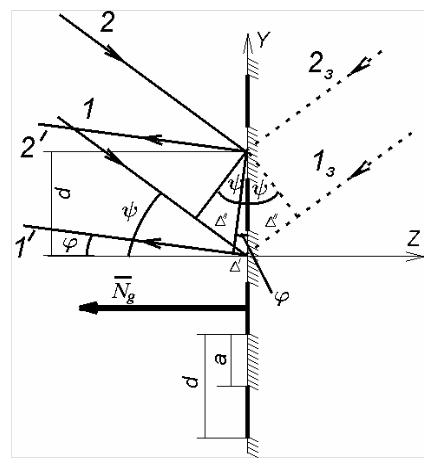
\includegraphics[width=0.5\textwidth]{1.png} 
    \caption{Дифракция на отражающей дифракционной решетке}
\end{figure}

\subsection{Автоколлимационный режим работы}
Частным случаем работы отражательной решетки является автоколлимация. В этом режиме падающий и дифрагированный лучи распространяются по одной и той же прямой во встречных направлениях.
\begin{itemize}
    \item \textbf{Условие:} Угол дифракции равен углу падения ($\varphi = \psi$).
Тогда  Уравнение решетки принимает вид:
    \begin{equation}
        2d \sin\varphi = k\lambda
    \label{eq:formula1}
    \end{equation}
\end{itemize}

\subsection{Профилированная решетка (эшелетт)}
Для устранения недостатка плоских решеток (концентрации большей части энергии в бесполезном нулевом порядке) применяются решетки с треугольным профилем штриха --- \textbf{эшелетты}.
\begin{itemize}
    \item Каждый штрих расположен под углом $\alpha$ (углом скоса) к основной плоскости решетки.
    \item \textbf{Угол "блеска":} 
    Максимальная концентрация энергии в спектре достигается, когда направление дифрагированного луча совпадает с направлением луча, зеркально отраженного от рабочей грани штриха.
    \item В автоколлимационном режиме условие блеска выполняется, когда свет падает по нормали к грани штриха. В этом случае угол дифракции равен углу скоса штриха: $\varphi = \alpha$.
\end{itemize}

\begin{figure}[H]
    \centering
    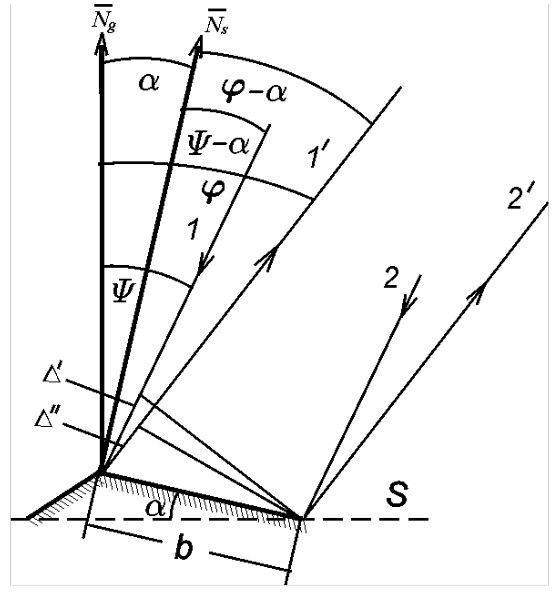
\includegraphics[width=0.4\textwidth]{2.png}
    \caption{Эшелетт. Дифракция на наклонном штрихе}
\end{figure}

\subsection{Основные характеристики спектрографа}

\textbf{1. Угловая дисперсия ($D_\varphi$)} --- характеризует угловое расстояние между лучами, отличающимися по длине волны на единицу:
\begin{equation}
    D_\varphi = \frac{\partial\varphi}{\partial\lambda} = \frac{k}{d \cos\varphi}
\end{equation}

\textbf{2. Линейная дисперсия ($D_l$)} --- определяет расстояние $dl$ на фокальной плоскости между спектральными линиями с разностью длин волн $d\lambda$:
\begin{equation}
    D_l = \frac{dl}{d\lambda} = F_2 \cdot D_\varphi = \frac{F_2 \cdot k}{d \cos\varphi}
\end{equation}
где $F_2$ --- фокусное расстояние камерного объектива. Часто используется \textit{обратная линейная дисперсия} ($d\lambda / dl$).

\textbf{3. Разрешающая способность ($R$)} --- способность прибора разделять две близкие спектральные линии (по критерию Рэлея):
\begin{equation}
    R = \frac{\lambda}{\delta\lambda} = k N
\end{equation}
где $N$ --- полное число освещенных штрихов решетки, $\delta\lambda$ --- минимально разрешимый интервал длин волн. Разрешение зависит только от порядка дифракции и числа штрихов.

\subsection{Духи Роуланда}
\textbf{Духи Роуланда} --- ложные спектральные линии, возникающие при использовании нарезных дифракционных решеток из-за периодической погрешности шага ходового винта делительной машины.

\textbf{Основные свойства:}
\begin{itemize}
    \item Образуют симметричные пары вокруг интенсивной («материнской») спектральной линии.
    \item Состоят из света той же длины волны $\lambda$, что и основная линия.
    \item Их относительная интенсивность стремительно возрастает пропорционально квадрату порядка дифракции ($\sim k^2$).
\end{itemize}

Смещение «духа» от основной спектральной линии описывается формулой:
\begin{equation}
    \Delta\lambda_R = \lambda \frac{m_R}{n_R}
\end{equation}
Где:
\begin{itemize}
    \item $\Delta\lambda_R$ --- расстояние по длинам волн от основной линии до ложной.
    \item $m_R$ --- порядок «духа».
    \item $n_R$ --- число штрихов, нарезаемых делительной машиной за один оборот ходового винта (параметр изготовления решетки).
\end{itemize}

\section{Эксперинтальная установка}
Данная лабораторная работа разделена на две части. \\
Первая из них --- изучение дифракции на прямоугольном от-
верстии.
\subsection{Первая часть работы}
\begin{figure}[H]
    \centering
    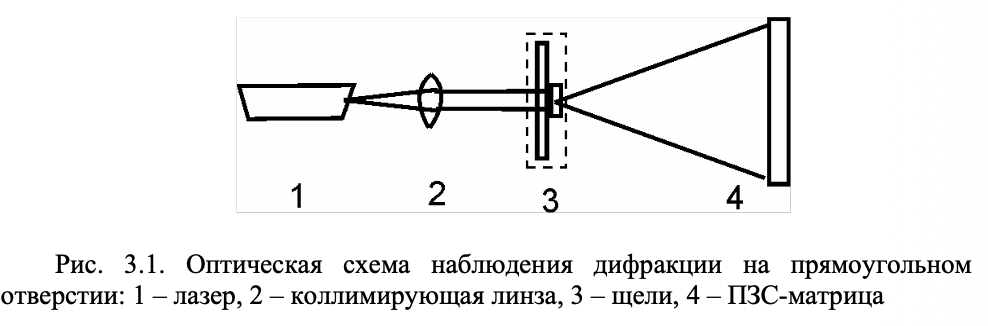
\includegraphics[width=0.9\textwidth]{3.png}
    \caption{Схема экспериментальной установки первой части работы}
\end{figure}

\subsubsection{Оптическая схема и элементы установки}
\begin{itemize}
    \item \textbf{Исследуемый объект:} Прямоугольное отверстие. Образовано двумя взаимно перпендикулярными щелями, расположенными вплотную. 
    \item \textbf{Регулировка:} Размеры прямоугольника (от узкой щели до квадрата) изменяются независимо с помощью двух микрометрических винтов.
    \item \textbf{Источник света:} Полупроводниковый лазерный диод. 
    \begin{itemize}
        \item Длина волны: $\lambda = 636$~нм
    \end{itemize}
\end{itemize}

\subsubsection{Система регистрации}
Дифракционная картина проецируется на ПЗС-матрицу видеокамеры и выводится на монитор компьютера.
\begin{itemize}
    \item \textbf{Параметры ПЗС-матрицы:}
    \begin{itemize}
        \item Разрешение: $760 \times 480$ пикселей.
        \item Линейные физические размеры: $5 \times 4$~мм$^2$.
    \end{itemize}
    \item \textbf{Геометрия установки:}
    \begin{itemize}
        \item Расстояние от отверстия до приемника (ПЗС-матрицы): $L = 105$~мм.
        \item Угловой размер приемника по горизонтали: $\approx 0.05$~рад.
    \end{itemize}
    \item \textbf{Принцип измерений:} Между физическим размером матрицы и изображением на мониторе существует строгая линейная зависимость. Измеряя линейное расстояние на экране монитора, с помощью коэффициента пересчета определяют реальное угловое расхождение лучей.
\end{itemize}

\subsection{Вторая часть работы}

Лабораторная установка представляет собой спектрометр (спектрограф), собранный по \textbf{автоколлимационной схеме} (схеме Игла). Особенность данной схемы заключается в том, что свет падает на дифракционную решетку и отражается от нее практически в одном и том же направлении, а один и тот же оптический элемент выполняет роль и коллиматора, и камеры.

\subsubsection{Основные оптические узлы установки}

\begin{itemize}
    \item \textbf{Источник излучения:} Ртутная лампа. Дает четкий линейчатый спектр (для измерений используется синяя линия триплета ртути $\lambda = 4358.3 \text{ \AA}$).
    \item \textbf{Осветитель (конденсор):} Линза, которая фокусирует свет от источника на входную щель прибора.
    \item \textbf{Входная щель:} Имеет регулируемую ширину. Служит точечным источником света для коллиматора. Ширина щели влияет на светосилу и разрешающую способность прибора.
    \item \textbf{Объектив (сферическое зеркало):} Выполняет двойную функцию:
    \begin{enumerate}
        \item Преобразует расходящийся пучок от входной щели в параллельный (работает как коллиматор).
        \item Собирает параллельный пучок, дифрагированный от решетки, фокусируя его в плоскости регистрации (работает как камерный объектив).
    \end{enumerate}
    \item \textbf{Диспергирующий элемент:} Отражательная профилированная дифракционная решетка (эшелетт) с периодом $d = 1/600$ мм. 
    \item \textbf{Система наблюдения/регистрации:} Экран + камера с измерительным перекрестием для наблюдения спектральных линий в фокальной плоскости.
\end{itemize}

\begin{figure}[H]
    \centering
    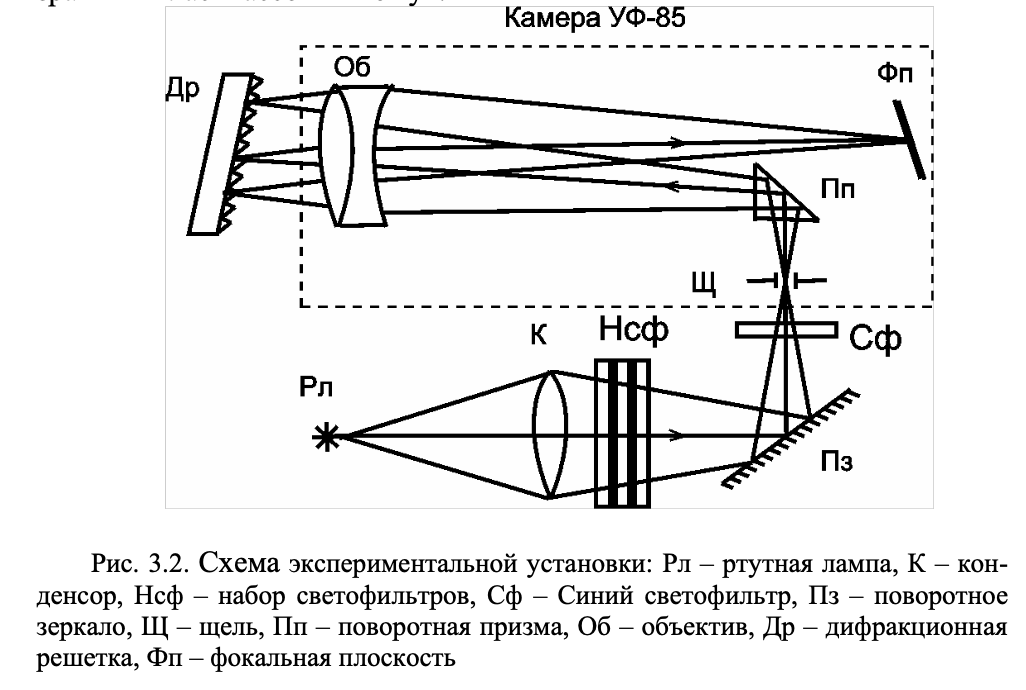
\includegraphics[width=0.9\textwidth]{4.png} 
    \caption{Оптическая (автоколлимационная) схема спектрометра}
\end{figure}

\subsubsection{Механизмы управления и измерения}

Для выполнения измерений установка снабжена точными механическими узлами:

\begin{itemize}
    \item \textbf{Поворотный столик с лимбом:} На нем закреплена дифракционная решетка. Вращение столика позволяет менять угол падения/дифракции $\varphi$ и выводить на экран различные порядки спектра. Угол отсчитывается по шкале лимба.
    \item \textbf{Микрометрический винт барабана (механизм поперечного смещения):} Служит для точного наведения измерительного перекрестия на спектральные линии. По шкале барабана снимаются отсчеты (в миллиметрах) для определения линейного расстояния $dl$ между линиями в фокальной плоскости (например, при расчете дисперсии и поиске духов Роуланда).
\end{itemize}

\section{Ход работы}
\subsection{Первая часть работы}
Изменяя ширину и длину прямоугольной щели, наблюдали различные картины. Ниже представлены некоторые примеры, полученные во время выполнения работы.
\begin{figure}[H]
    \centering
    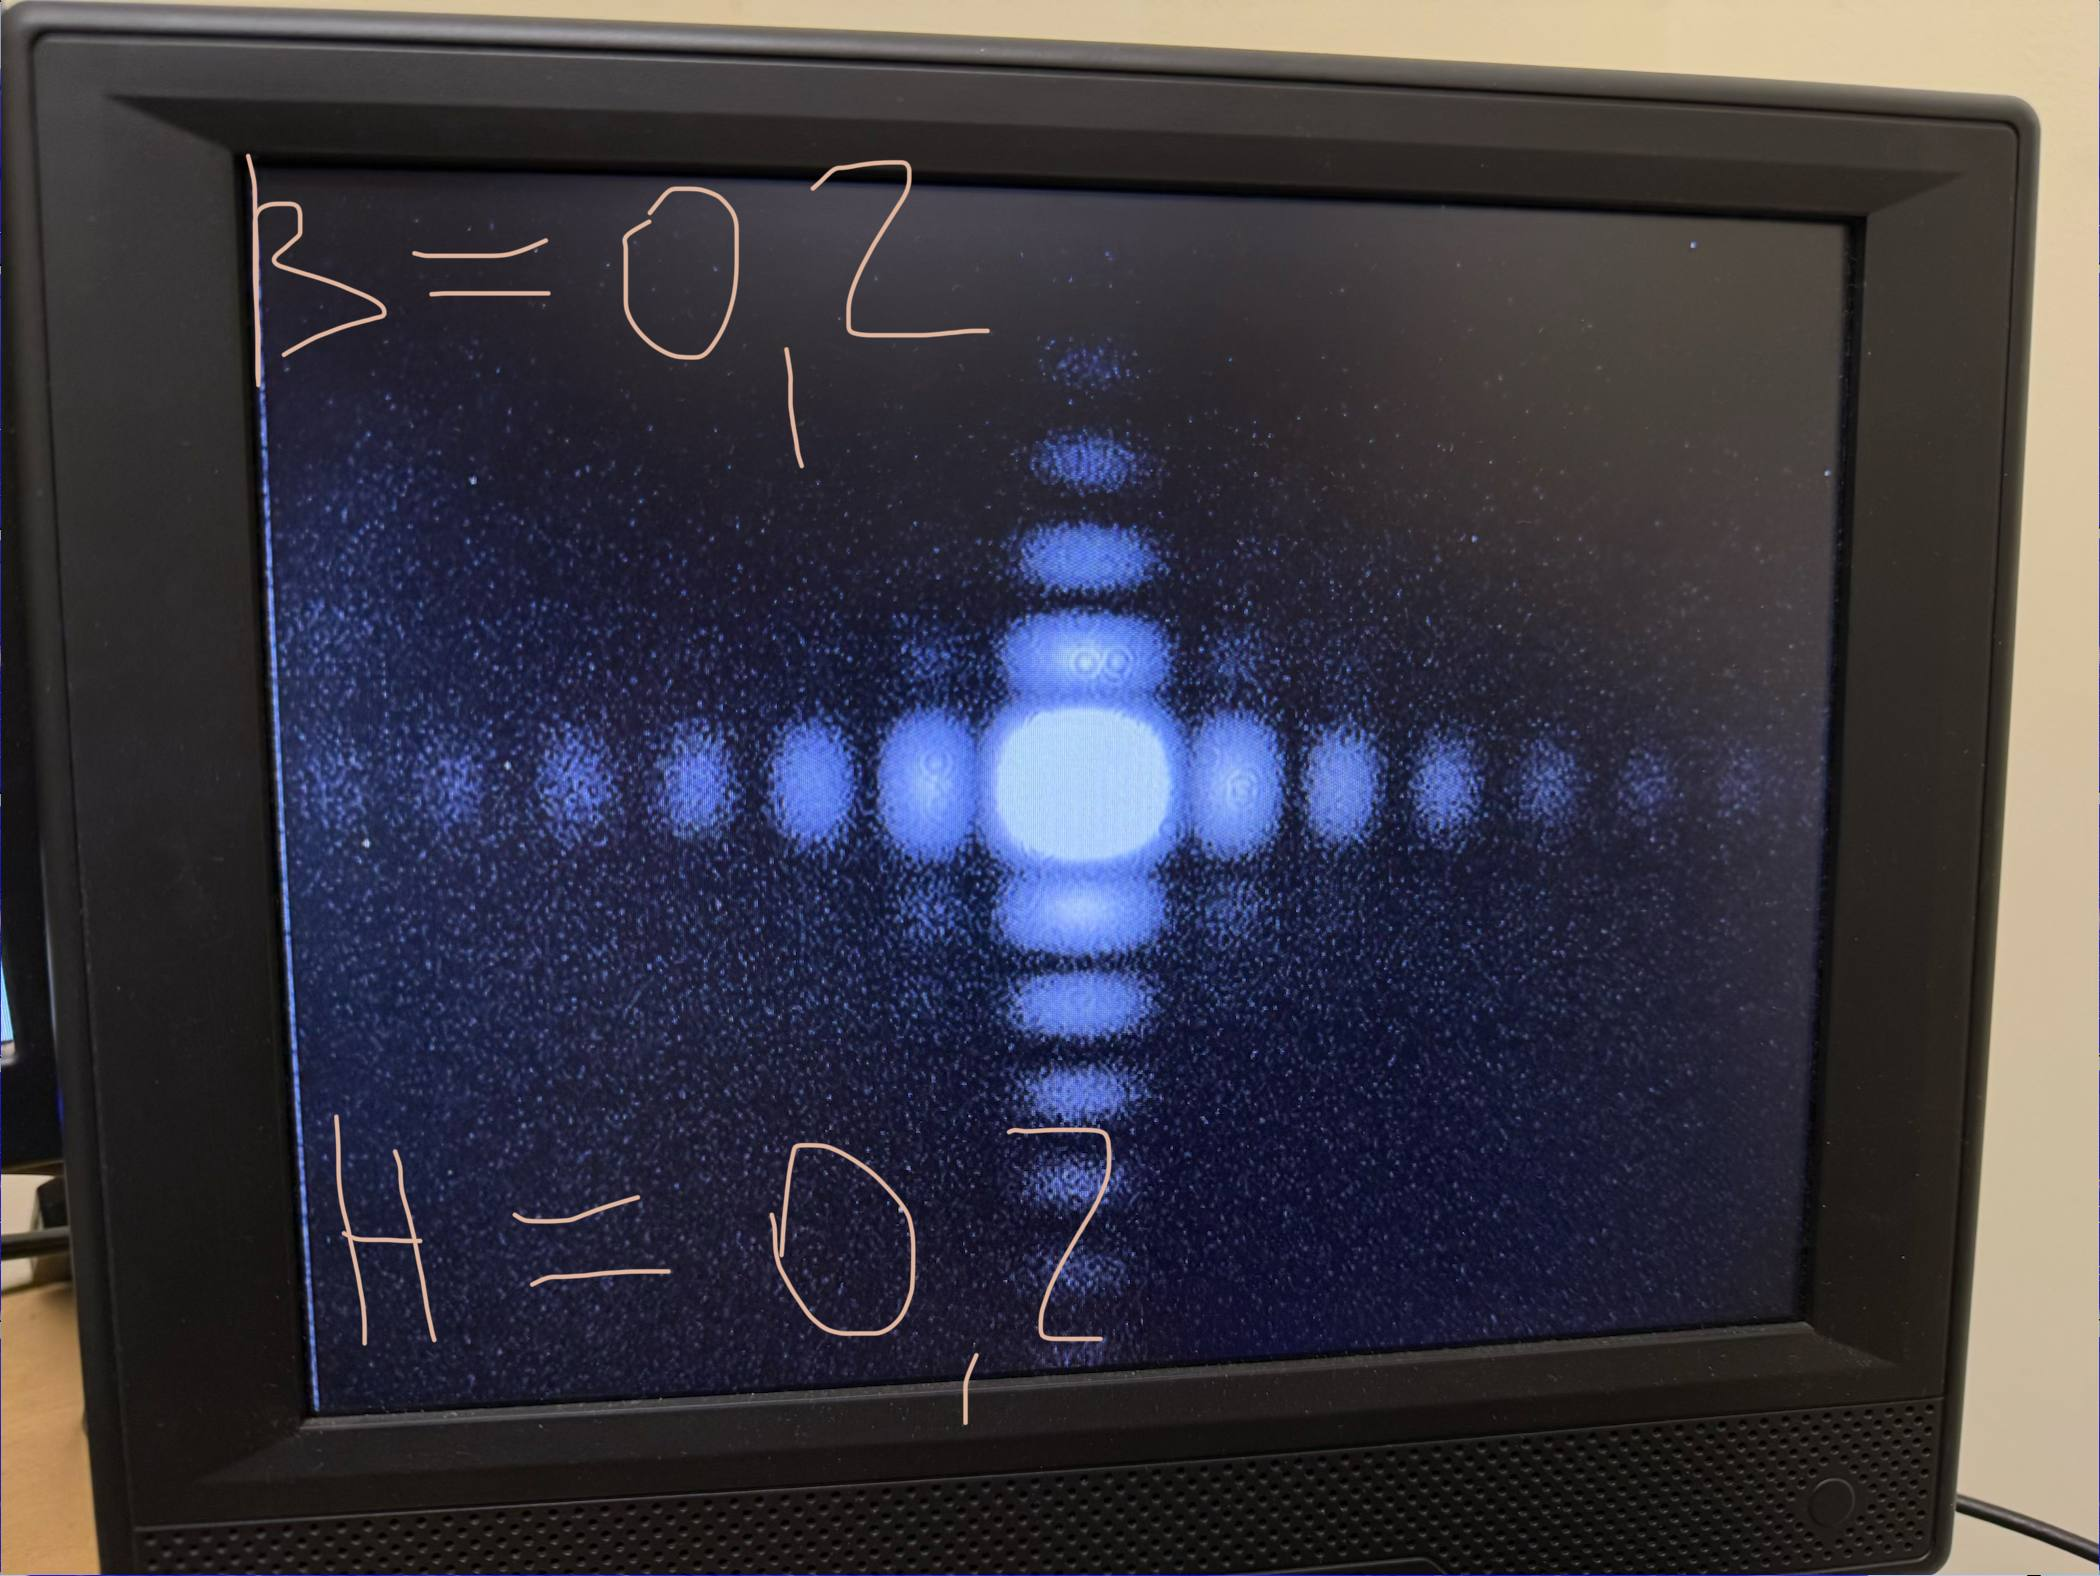
\includegraphics[width=0.5\textwidth]{11.JPG} 
    \caption{Картинка 1}
    \label{eq:11}
\end{figure}
\begin{figure}[H]
    \centering
    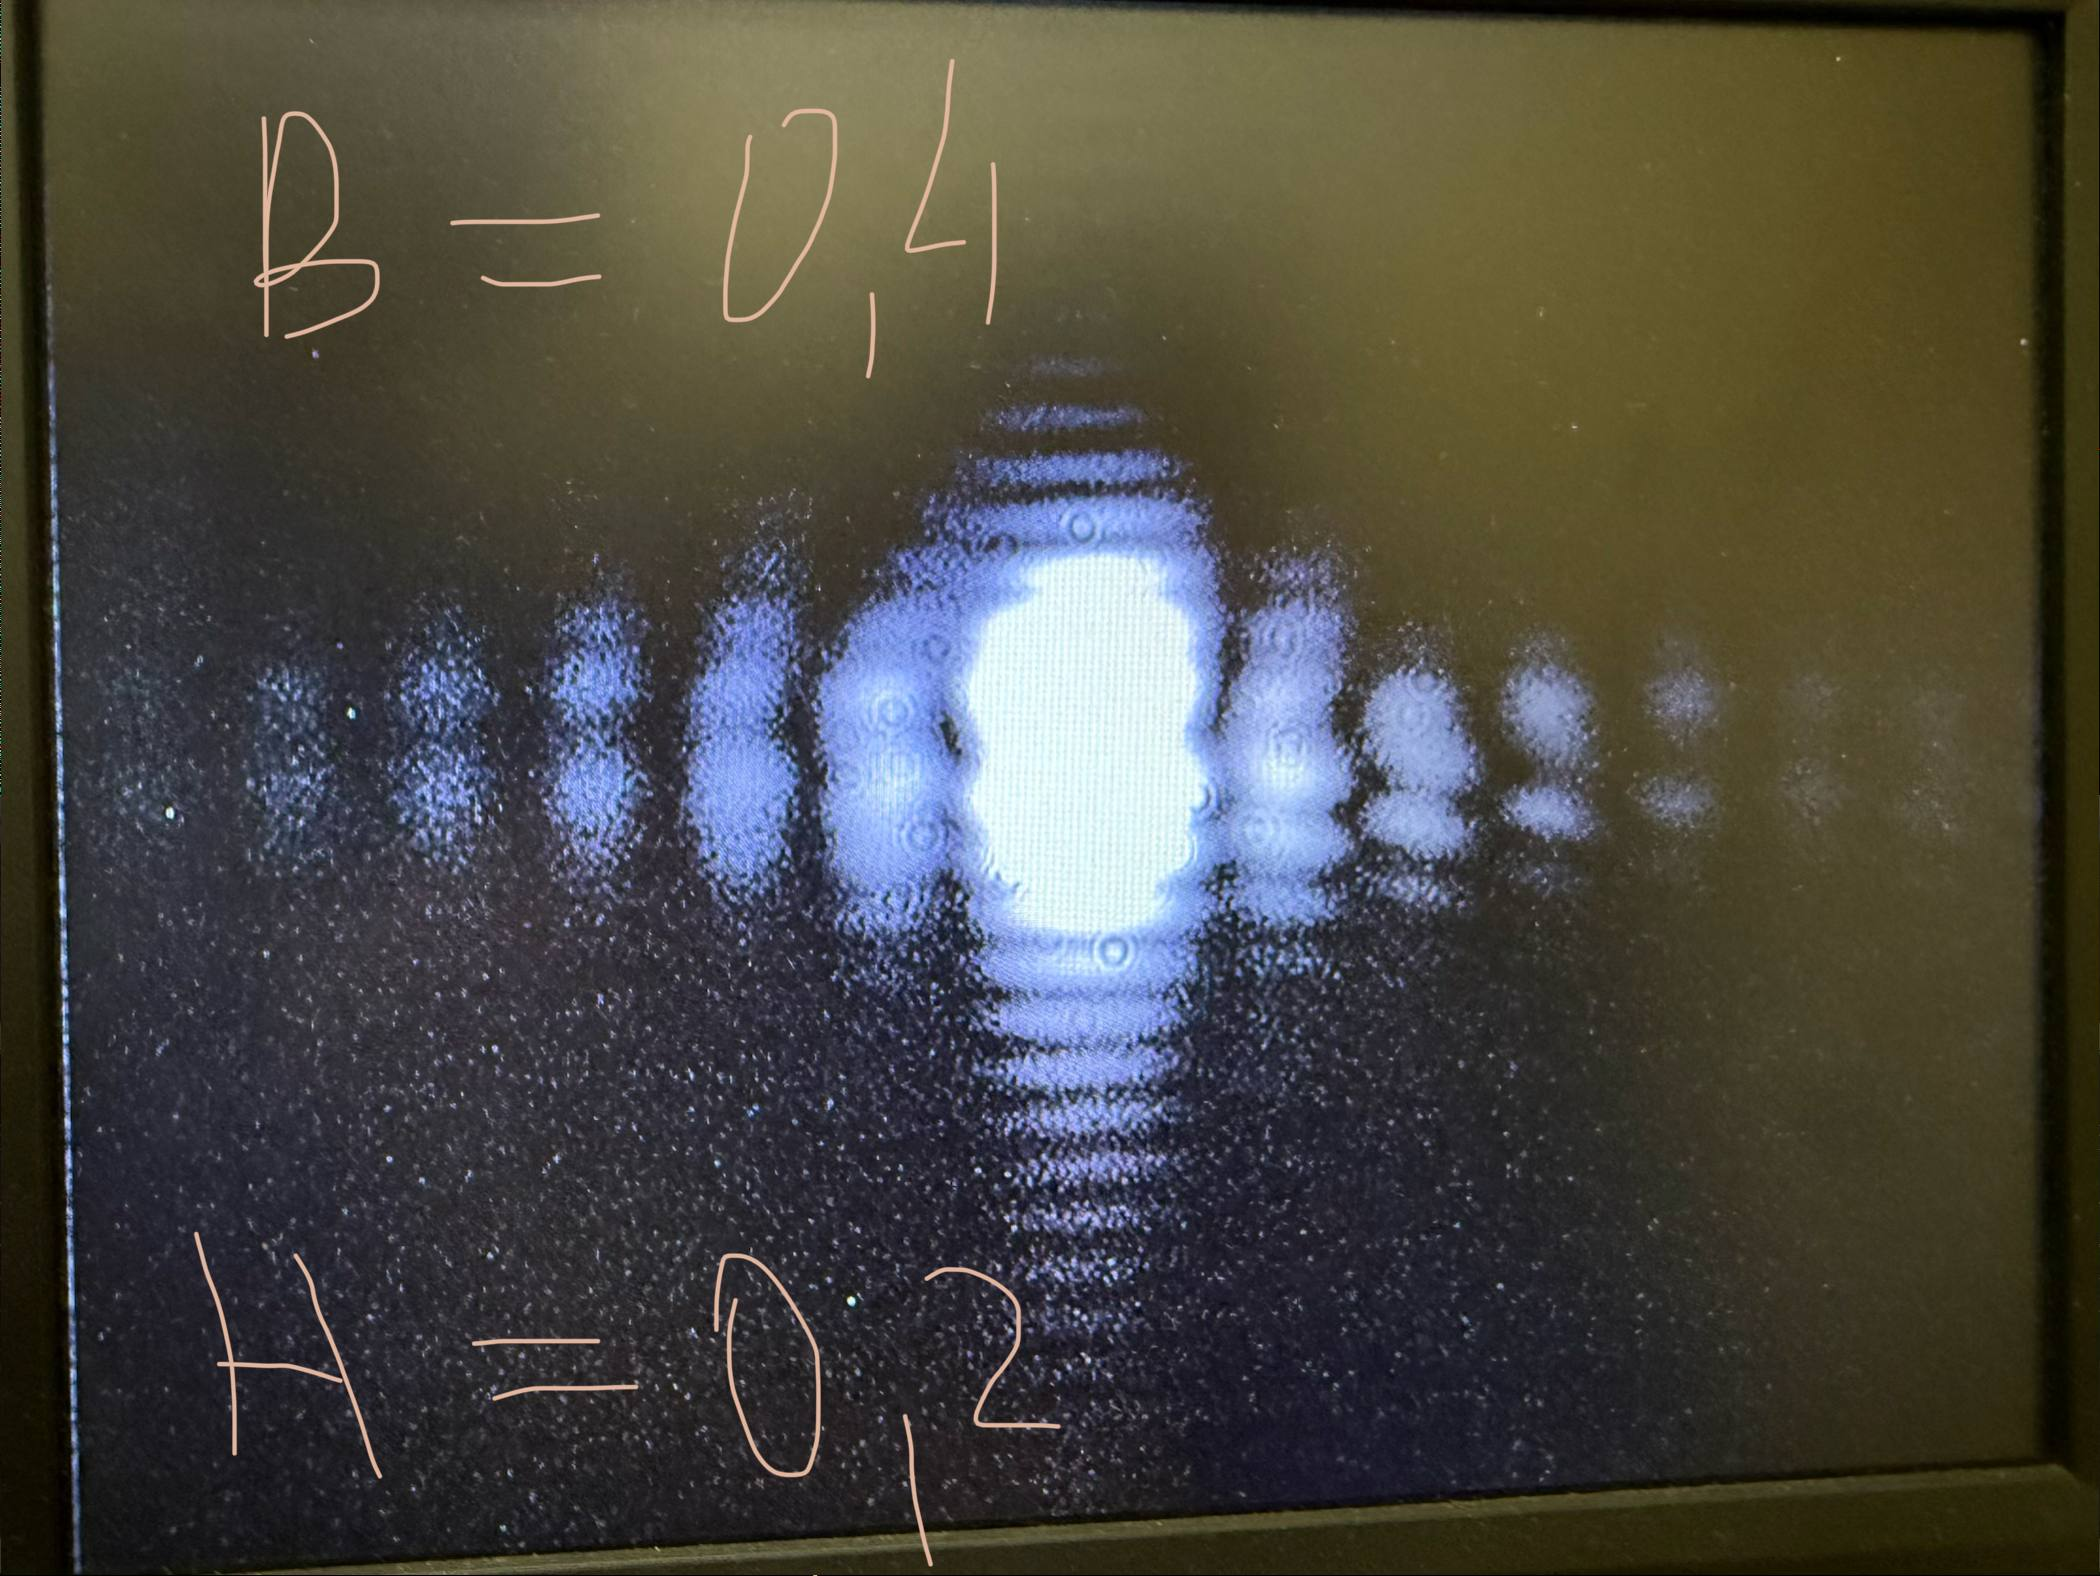
\includegraphics[width=0.5\textwidth]{12.JPG} 
    \caption{Картинка 2}
    \label{eq:12}
\end{figure}
\begin{figure}[H]
    \centering
    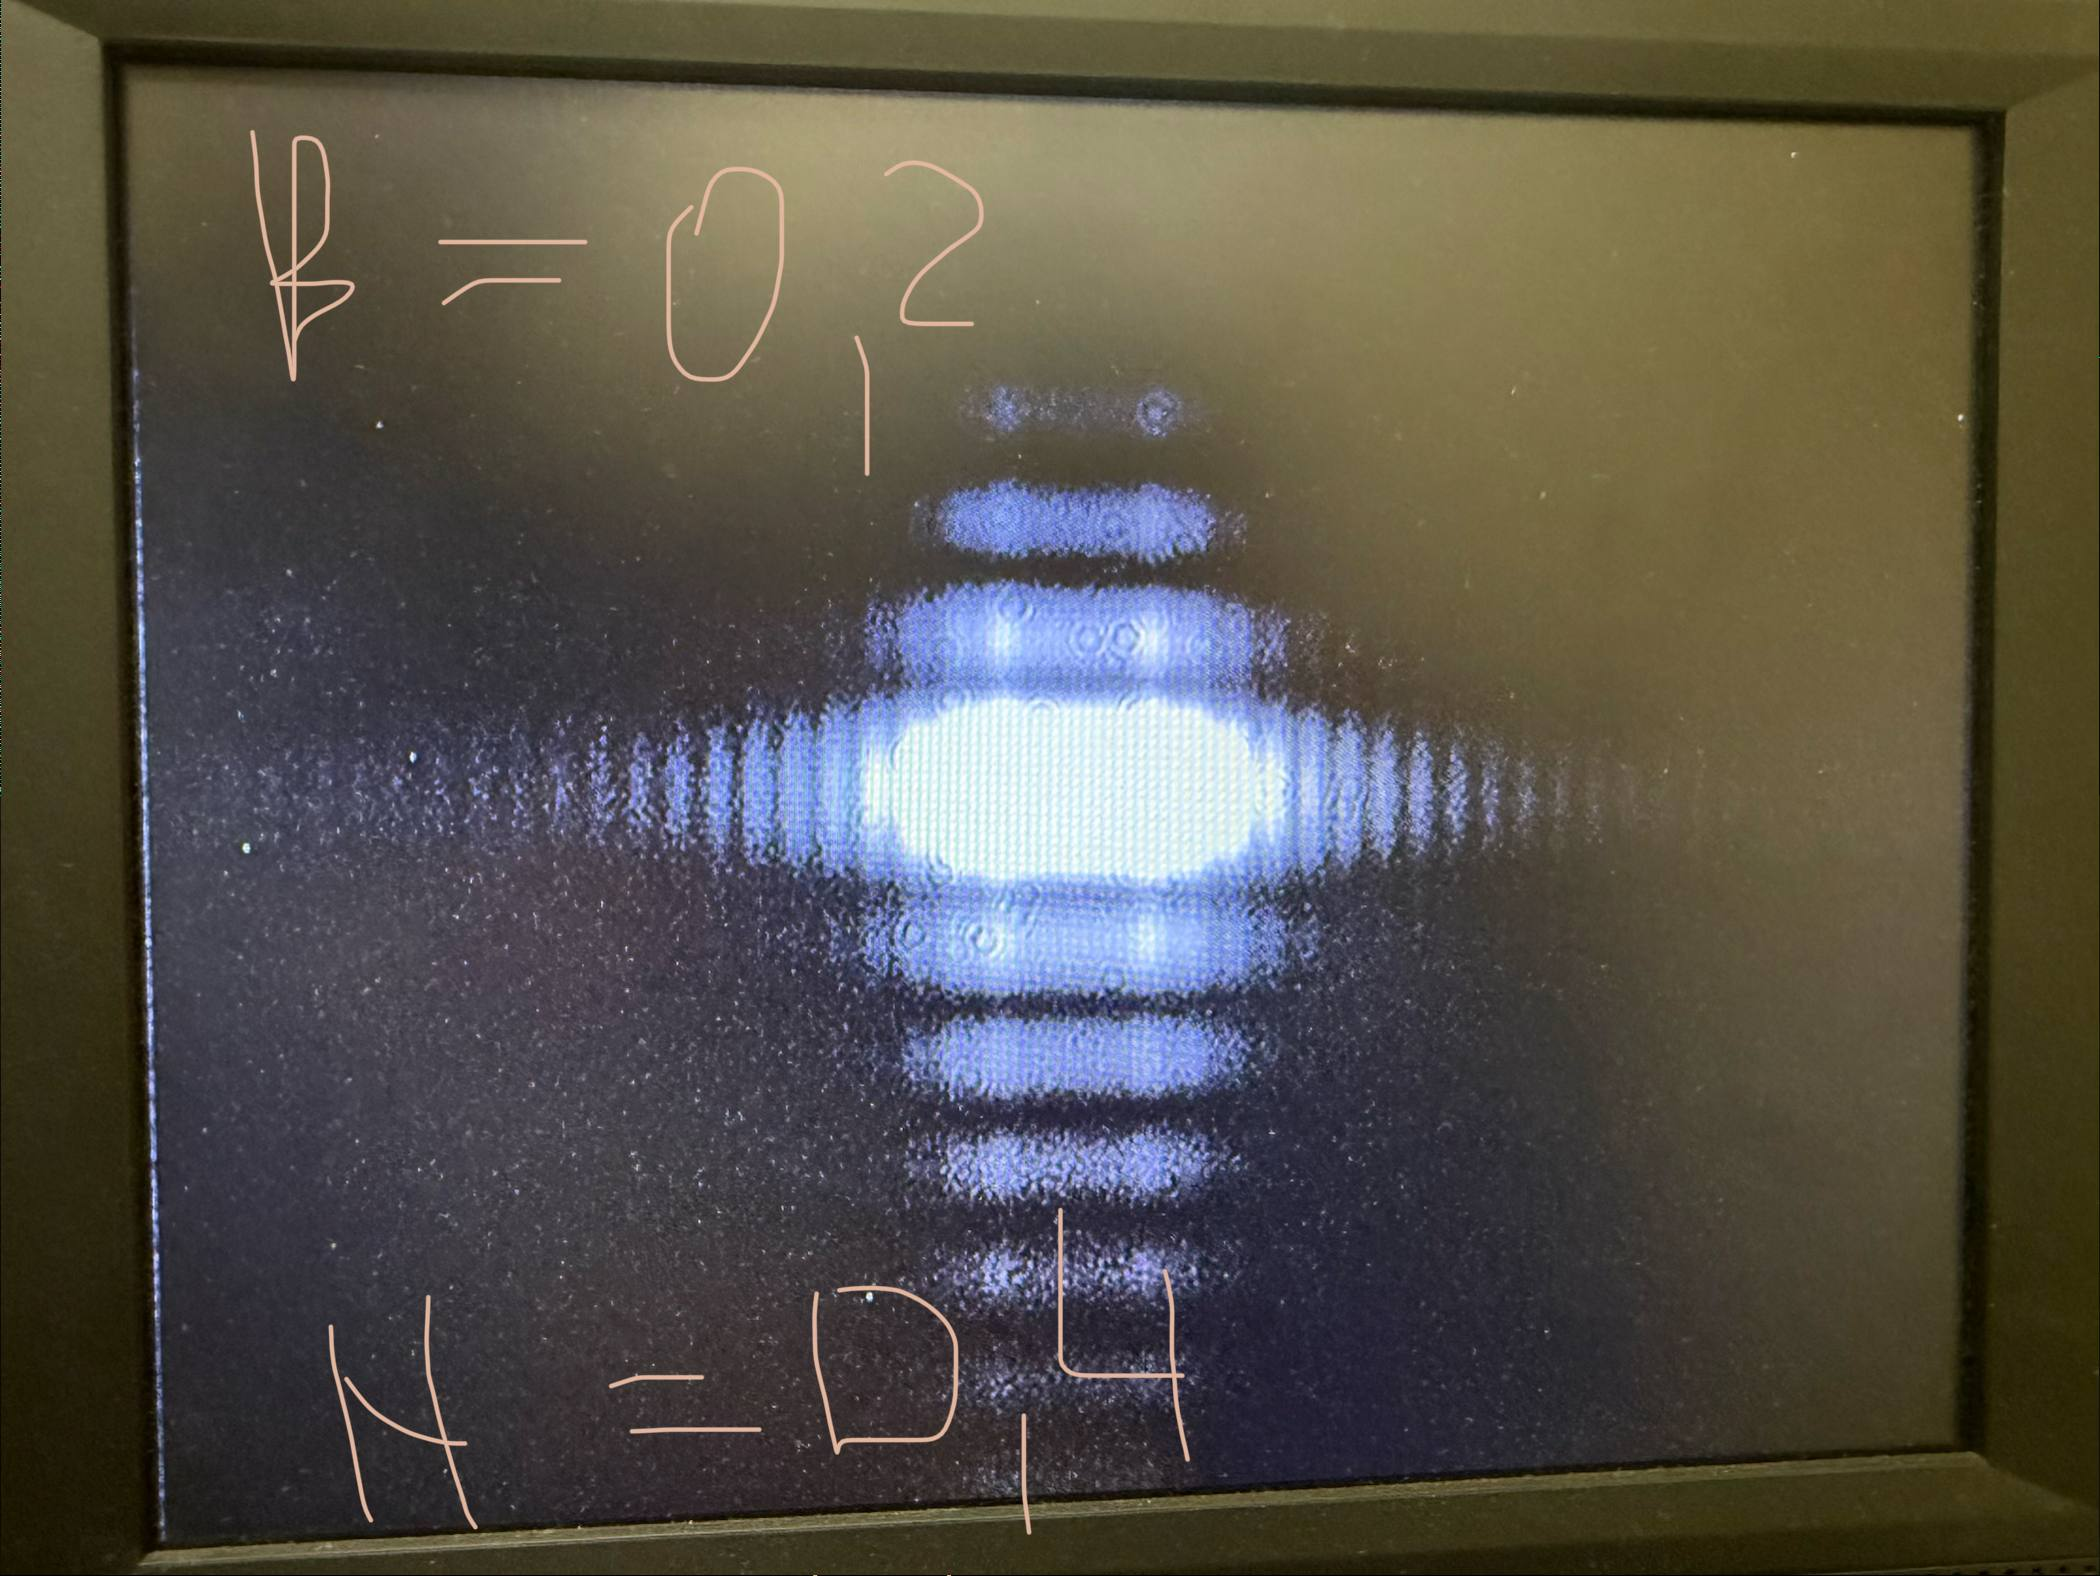
\includegraphics[width=0.5\textwidth]{13.JPG} 
    \caption{Картинка 3}
    \label{eq:13}
\end{figure} 
\\
На \ref{eq:11} --- 0.2*0.2 $\text{мм}^2$, на \ref{eq:12} --- 0.4*0.2 $\text{мм}^2$, на \ref{eq:13} --- 0.2*0.4 $\text{мм}^2$.

Измерили расстояние между минимумами около центрального максимума у щелей разных размеров, чтобы вычислить его угловой размер по параметрам установки. Посчитали теоретические значения по формуле:

\begin{equation}
    2\psi = \frac{2\lambda}{S_\text{щ}}
\end{equation}

Результаты приведены в таблице ниже:

\begin{table}[H]
\centering

\begin{tabular}{|c|c|c|c|}
\hline
$S_{\text{щ}},\,\text{мм}$ & $\Delta x,\,\text{мм}$ & $2\psi_{\text{эксп}}$, град & $2\psi_{\text{теор}}$, град \\
\hline
0.20 & 0.69 & 0.377 & 0.364 \\
\hline
0.25 & 0.46 & 0.251 & 0.292 \\
\hline
0.30 & 0.33 & 0.180 & 0.243 \\
\hline
0.35 & 0.31 & 0.169 & 0.208 \\
\hline
\end{tabular}

\caption{Экспериментальные и теоретические значения $2\psi$}
\end{table}
\newpage
По полученным данным построим график зависимости $2\psi$ от ширины щели.

\begin{figure}[H]
    \centering
    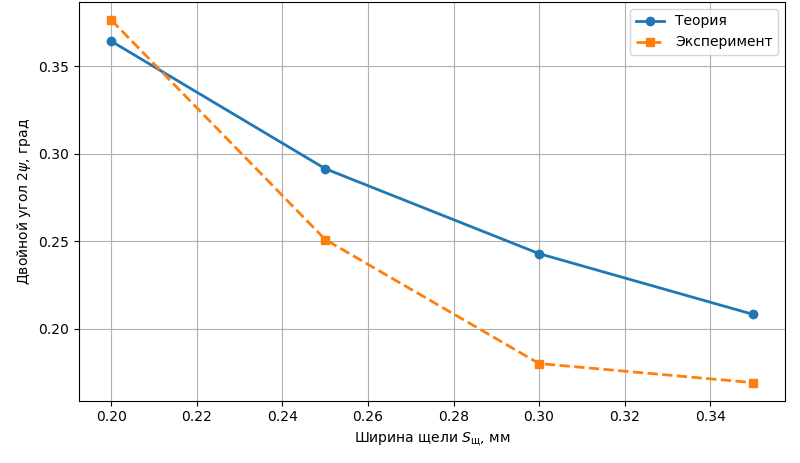
\includegraphics[width=0.75\linewidth]{out3.png}
    \caption{Зависимость ширины щели от углового размера главного максимума}
    \label{fig:chrom_aberr}
\end{figure}


\subsection{Вторая часть работы}
\subsubsection{Исследование хроматической аберрации
объектива камеры}
Вывели решетку на ахроматический порядок спектра.\\
Для каждой из линий, имеющихся в наборе светофильтров Нсф, выставили положение объектива таким образом, чтобы картинка на экране монитора была наиболее резкой. Результаты:
\begin{table}[H]
    \centering
    \label{tab:nsf}
    \footnotesize
    \begin{tabular}{|c|c|}
    \hline
    $\lambda$, нм & d, мм \\
    \hline
    579 & 112.0 \\
    546 & 105.4 \\
    436 & 70.2 \\
    405 & 54.5 \\
    366 & 26.2 \\
    \hline
    \end{tabular}
    \caption{Зависимость положения объектива от длины падающей волны}
\end{table}


По результатам измерений была построена зависимость положения объектива камеры от длины волны излучения.

\begin{figure}[H]
    \centering
    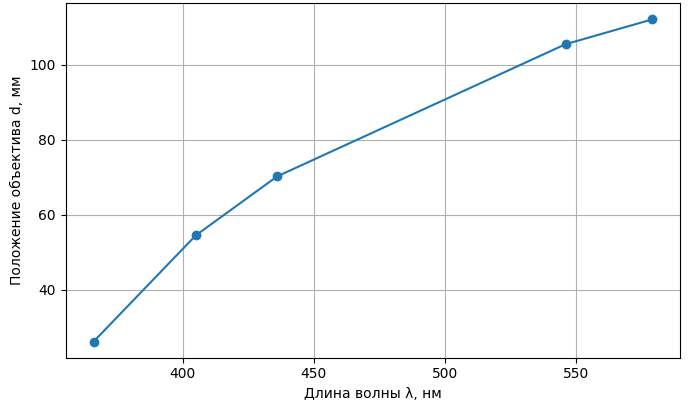
\includegraphics[width=0.75\linewidth]{output.png}
    \caption{Зависимость положения объектива камеры от длины волны}
    \label{fig:chrom_aberr}
\end{figure}

По графику видно, что положение объектива, соответствующее наилучшей резкости изображения, зависит от длины волны. Это свидетельствует о наличии хроматической аберрации объектива камеры.

\subsubsection{Определение углов дифракции}
Закрепили светофильтр Сф на оправе входной щели.
По формуле \ref{eq:formula1} произвели расчёт углов поворота решётки для левых и правых максимумов.
\begin{itemize}
    \item \textbf{Длина волны:} Для расчетов используется синяя линия спектра ртути $\lambda = 4358.3 \text{ \AA}$.
    \item \textbf{Период решетки:} $d = 1/600 \text{ мм}$. 
    Переведем в ангстремы для согласования размерностей: 
    $d = 1.6667 \cdot 10^{-3} \text{ мм} = 16666.7 \text{ \AA}$.
\end{itemize}

Вычислим постоянный множитель для нашей решетки и длины волны:
\begin{equation*}
    \frac{\lambda}{2d} = \frac{4358.3}{2 \cdot 16666.7} = \frac{4358.3}{33333.4} \approx 0.130749
\end{equation*}

Подставляя значения $k$ от 0 и выше, найдем углы поворота решетки $\varphi_k$. Знак $\pm$ указывает на симметричные левый и правый порядки.

\begin{itemize}
    \item \textbf{Нулевой порядок ($k = 0$):} \\
    $\sin\varphi_0 = 0 \quad \Rightarrow \quad \mathbf{\varphi_0 = 0^\circ}$
    
    \item \textbf{Первый порядок ($k = \pm 1$):} \\
    $\sin\varphi_1 = 1 \cdot 0.130749 \approx 0.1307 \quad \Rightarrow \quad \mathbf{\varphi_1 \approx 7^\circ 31'}$
    
    \item \textbf{Второй порядок ($k = \pm 2$):} \\
    $\sin\varphi_2 = 2 \cdot 0.130749 \approx 0.2615 \quad \Rightarrow \quad \mathbf{\varphi_2 \approx 15^\circ 10'}$
    
    \item \textbf{Третий порядок ($k = \pm 3$):} \\
    $\sin\varphi_3 = 3 \cdot 0.130749 \approx 0.3922 \quad \Rightarrow \quad \mathbf{\varphi_3 \approx 23^\circ 05'}$
    
    \item \textbf{Четвертый порядок ($k = \pm 4$):} \\
    $\sin\varphi_4 = 4 \cdot 0.130749 \approx 0.5230 \quad \Rightarrow \quad \mathbf{\varphi_4 \approx 31^\circ 32'}$
\end{itemize}

Нулевой порядок дифракции наблюдается при угле поворота решётки $85^\circ$ (нулевой угол).

Затем, производим последовательный вывод на середину экрана наиболее сильную линию ртути в первом порядке спектра, манипулируя
грубым и точным устройствами поворота решетки. \\
Зафиксировали отсчёт по лимбу от нулевого угла:
% Вставь, пж, все данные
\begin{table}[H]
\centering
\begin{tabular}{|c|c|}
\hline
Порядок $k$ & Угол дифракции, град \\
\hline
$-3$ & $-23^\circ$ \\
$-2$ & $-15^\circ$ \\
$-1$ & $-7^\circ$ \\
$0$  & $0^\circ$ \\
$1$  & $8^\circ$ \\
$2$  & $15^\circ$ \\
$3$  & $23.5^\circ$ \\
\hline
\end{tabular}
\caption{Экспериментально определённые углы дифракции относительно нулевого порядка}
\end{table}


Качественно сравнивая яркость изображения линий на экране монитора определили порядок дифракции с наибольшей концентрацией
энергии - это первый порядок. Угол скоса грани штриха эшелетта – $\alpha \approx 7^\circ 31'$.

\subsubsection{Измерение линейной дисперсии}
Для правых первого, второго и третьего максимумов вращением микрометрического винта угла поворота решётки на это же деление монитора, выводим вторую – $\lambda_2$ и третью – $\lambda_3$ линии триплета, отсчитывая угол поворота решетки по лимбу.
Результаты - ниже: \\

\begin{table}[H]
\centering
 \renewcommand{\arraystretch}{1.5}
    \resizebox{\columnwidth}{!}{

\begin{tabular}{|c|c|c|c|}
\hline
Порядок спектра $k$ & $\lambda_1 = 4358{,}3\,\text{\AA},\ \varphi_1$ & $\lambda_2 = 4347{,}5\,\text{\AA},\ \varphi_2$ & $\lambda_3 = 4339{,}2\,\text{\AA},\ \varphi_3$ \\
\hline
1 & $6.970^\circ$  & $6.936^\circ$  & $6.904^\circ$  \\
\hline
2 & $15.147^\circ$ & $15.071^\circ$ & $15.006^\circ$ \\
\hline
3 & $23.128^\circ$ & $23.009^\circ$ & $22.917^\circ$ \\
\hline
\end{tabular}
}
\caption{Значения углов дифракции для линий триплета}
\end{table}

По ним можно вычислить угловую дисперсию в первом порядке и
рассчитать линейную дисперсию: \\
\begin{table}[H]
    \centering
    \renewcommand{\arraystretch}{1.5}
    \resizebox{\columnwidth}{!}{
    \begin{tabular}{|c|c|c|c|}
        \hline
        \textbf{Порядок} & \textbf{Угол дифракции} & \textbf{Угловая дисперсия} & \textbf{Обратная лин. дисперсия} \\
        $k$ & $\varphi_k$, град & $D_\varphi = \frac{d\varphi}{d\lambda}$, $10^{-4}$ рад/\AA & $\frac{d\lambda}{dl}$, \AA/мм \\
        \hline
        1 & $6.936^\circ$ & 0.603 & 12.75 \\
        \hline
        2 & $15.071^\circ$ & 1.288 & 5.97 \\
        \hline
        3 & $23.009^\circ$ & 1.928 & 3.99 \\
        \hline
    \end{tabular}
    }
    \caption{Экспериментальные значения дисперсии для различных порядков спектра}
\end{table}
\newpage
По полученным данным построим графики зависимости угловой дисперсии $d\varphi/d\lambda$ и обратной линейной дисперсии $d\lambda/dl$ от угла поворота решетки. \\

\begin{figure}[H]
    \centering
    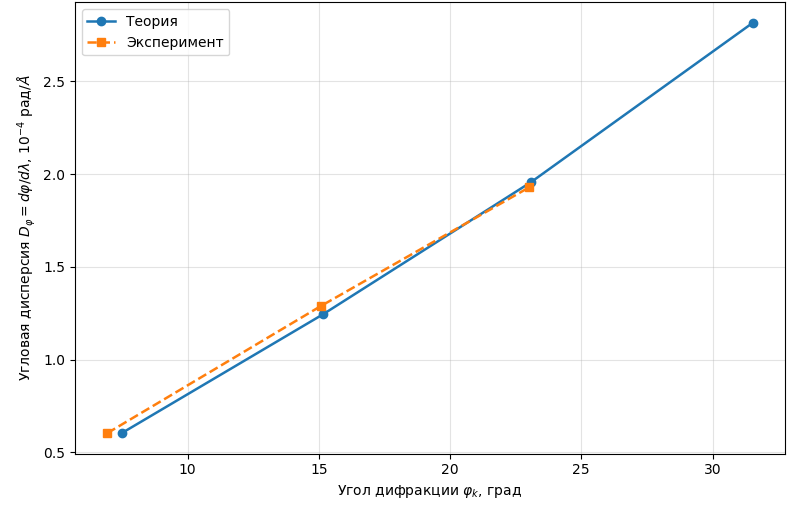
\includegraphics[width=0.75\linewidth]{out1.png}
    \caption{Зависимость угловой дисперсии от угла дифракции}
    \label{fig:chrom_aberr}
\end{figure}


\begin{figure}[H]
    \centering
    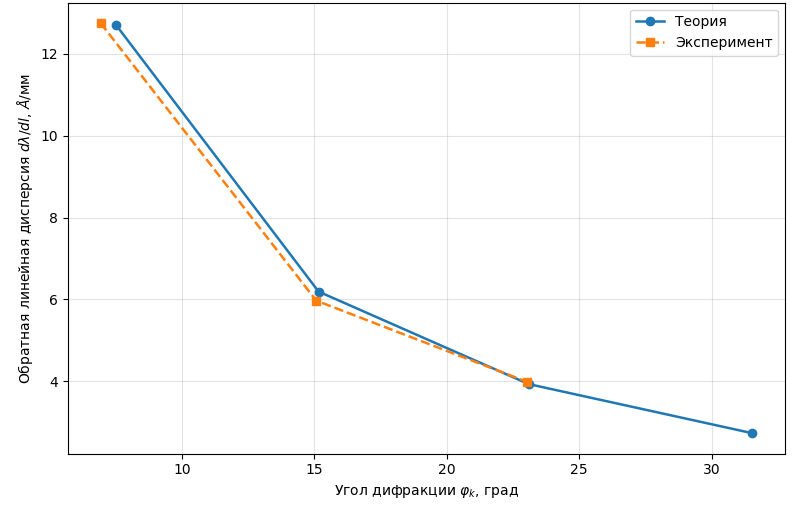
\includegraphics[width=0.75\linewidth]{out2.png}
    \caption{Зависимость обратной линейной дисперсии от угла дифракции}
    \label{fig:chrom_aberr}
\end{figure}
\newpage
Сравним полученное с теорией.\\
Воспользуемся следующей формулой: \\
\begin{equation}
    \frac{d\lambda}{dl} = \frac{1}{D_l} = \frac{1}{F_2 \cdot D_\varphi} = \frac{d \cos\varphi_k}{k \cdot F_2} \quad \left[ \frac{\text{\AA}}{\text{мм}} \right]
\end{equation}

Для расчетов подставим константы в формулу обратной линейной дисперсии:
\begin{equation*}
    \frac{d\lambda}{dl} = \frac{16666.7 \cdot \cos\varphi_k}{1300 \cdot k} \approx 12.82 \cdot \frac{\cos\varphi_k}{k} \quad \left[ \frac{\text{\AA}}{\text{мм}} \right]
\end{equation*}

Используя углы дифракции $\varphi_k$, рассчитанные ранее для линии $\lambda = 4358.3 \text{ \AA}$, вычислим значения дисперсий для всех доступных порядков.

\begin{table}[H]
    \centering
    \renewcommand{\arraystretch}{1.5}
    \resizebox{\columnwidth}{!}{
    \begin{tabular}{|c|c|c|c|c|}
        \hline
        \textbf{Порядок} & \textbf{Угол дифракции} & \textbf{Косинус угла} & \textbf{Угловая дисперсия} & \textbf{Обратная лин. дисперсия} \\
        $k$ & $\varphi_k$, град & $\cos\varphi_k$ & $D_\varphi = \frac{d\varphi}{d\lambda}$, $10^{-4}$ рад/\AA & $\frac{d\lambda}{dl}$, \AA/мм \\
        \hline
        1 & $7.51^\circ$ & 0.9914 & 0.605 & 12.71 \\
        \hline
        2 & $15.16^\circ$ & 0.9652 & 1.244 & 6.19 \\
        \hline
        3 & $23.09^\circ$ & 0.9199 & 1.957 & 3.93 \\
        \hline
        4 & $31.53^\circ$ & 0.8524 & 2.815 & 2.73 \\
        \hline
    \end{tabular}
    }
    \caption{Теоретические значения дисперсии спектрографа для различных порядков спектра}
\end{table}

\subsubsection{Наблюдение «духов» Роуланда}
В четвёртом порядке произвели наблюдение духов Роуланла. Полученное смещение

\begin{table}[H]
\centering
 \renewcommand{\arraystretch}{1.5}
    \resizebox{\columnwidth}{!}{
\begin{tabular}{|c|c|c|c|c|}
\hline
Порядок $k$ & Угол основной линии, град & Угол духа, град & $\Delta \varphi$, град & $\Delta \lambda_R$, \AA \\
\hline
4 & $32.0^\circ$ & $29.5^\circ$ & $2.5^\circ$ & $163$ \\
\hline
\end{tabular}
}
\caption{Результаты наблюдения духа Роуланда в четвёртом порядке}
\end{table}

Смещение ``духа'' Роуланда от основной спектральной линии описывается формулой (6). Отсюда
\[
n_R = \frac{4358.3 \cdot 4}{163} \approx 107
\]

Следовательно, число штрихов, наносимых за один оборот колеса делительной машины, составляет
\[
\boxed{n_R \approx 107}
\]
%Данные, расчёты, бизнес, семья
\subsubsection{Расчет разрешающей способности}
%Там просто расчёты и графичек
Разрешающая способность дифракционной решётки определяется формулой
(5).

Полное число штрихов на всей рабочей ширине:
\[
N_{\text{реш}} = 150 \cdot 600 = 90000.
\]
Тогда для всей решётки:
\[
R_{\text{реш}} = k N_{\text{реш}} = 90000\,k.
\]

Объектив камеры УФ-85 имеет фокусное расстояние
\[
F = 1300\ \text{мм}
\]
и относительное отверстие \(1:25\). Следовательно, диаметр действующего пучка равен
\[
D = \frac{F}{25} = \frac{1300}{25} = 52\ \text{мм}.
\]
Число освещённых штрихов решётки в установке:
\[
N_{\text{уст}} = 52 \cdot 600 = 31200.
\]
Следовательно,
\[
R_{\text{уст}} = k N_{\text{уст}} = 31200\,k.
\]

Рассчитаем разрешающую способность для наблюдавшихся порядков спектра:

\begin{table}[H]
\centering
\begin{tabular}{|c|c|c|}
\hline
Порядок $k$ & $R_{\text{реш}}$ & $R_{\text{уст}}$ \\
\hline
1 & 90000 & 31200 \\
2 & 180000 & 62400 \\
3 & 270000 & 93600 \\
\hline
\end{tabular}
\caption{Теоретическая разрешающая способность для всей решётки и установки}
\end{table}

Построим график зависимости разрешающей способности от порядка дифракции:

\begin{figure}[H]
    \centering
    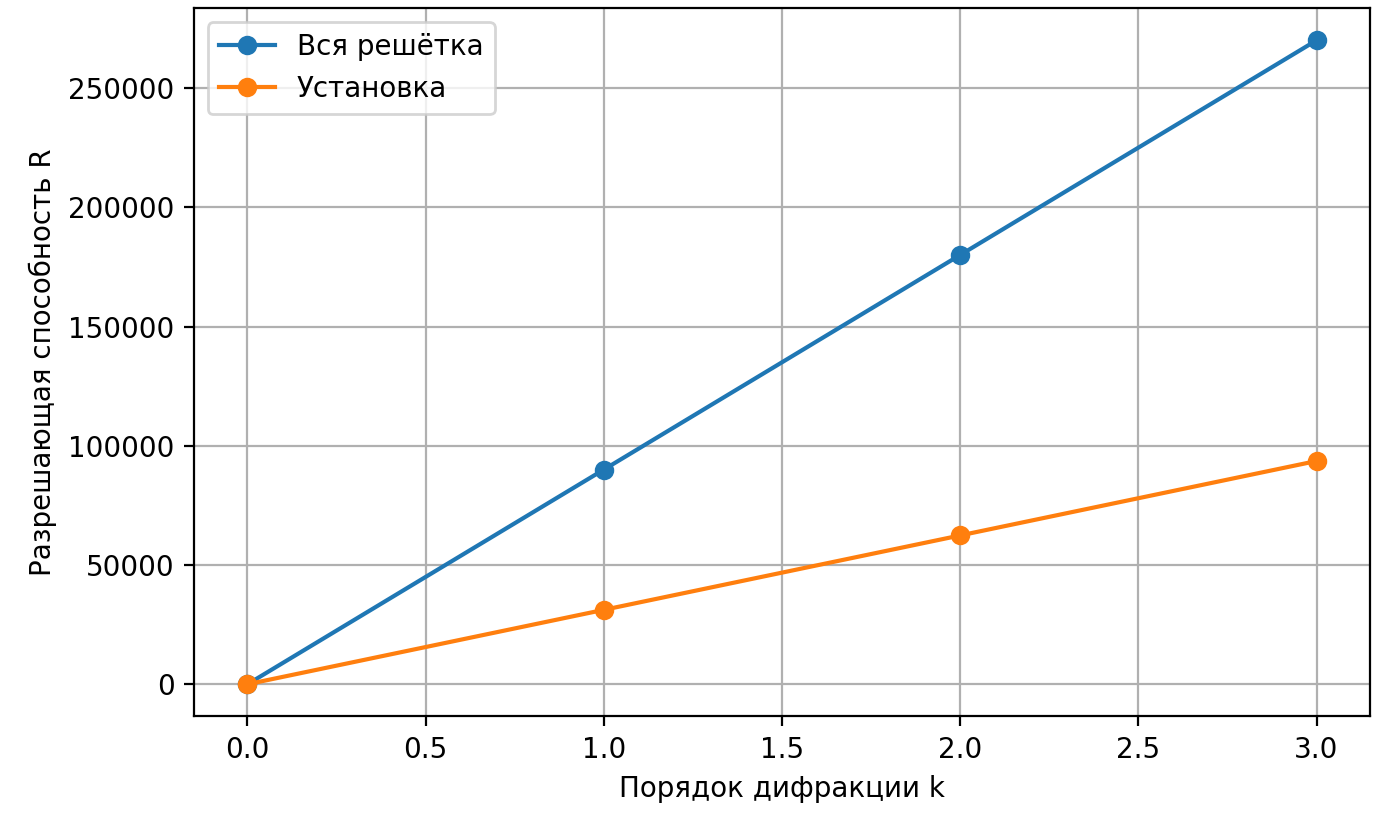
\includegraphics[width=0.75\linewidth]{output2.png}
    \caption{Зависимость разрешающей способности от порядка дифракции для всей решётки и для установки}
    \label{fig:resolution_power}
\end{figure} 
\newpage
\section{Вывод}
В данной работе были изучены основы дифракции света, спектрографии и устройства спектральных приборов, а также произведено исследование данных дифракционных решёток.
\end{document} 
